\documentclass[11pt,a4paper]{article}
\usepackage[utf8]{inputenc}
\usepackage{amsmath}
\usepackage{amsfonts}
\usepackage{amssymb}
\usepackage{blindtext}
\usepackage{graphicx}
\usepackage{subcaption}
\usepackage{wrapfig}
\usepackage[font=small,labelfont=bf]{caption}
\graphicspath{ {./images/} }
\captionsetup[figure]{name = Abbildung}
\captionsetup[table]{name = Tabelle}
\renewcommand{\refname}{Literatur}

\begin{document}
\title{Blumenklassifikation anhand von Blüten: Ein Vergleich von Farb- und HOG-Merkmalen mit CNNs}
\author{Aaron Eisermann, Franziska Eder, Georg Siemund}
\maketitle

\begin{abstract}
Diese Arbeit vergleicht verschiedene Ansätze zur Klassifikation von Pflanzenarten. Hierbei wird die Pflanze anhand der Blüte als Hauptmerkmal in eine von 10 Klassen eingeordnet. Wir haben als Deskriptoren HOGs, Farb-Histogramme, Farbmittelwerte und die Kombination aller Methoden untersucht. Darüber hinaus haben wir die Klassifikation mittels eines großen, vortrainierten Deep Convolutional Neural Network (CNN) untersucht, dem VGG-16. Der zugrundeliegende Datensatz entstammt einer Oxford-Studie. Dem umfangreichen Datensatz haben wir zufällig 10 Klassen mit jeweils 40 Bildern entnommen. Wir kommen zu dem Schluss, dass das VGG-CNN, das eine Genauigkeit von bis zu 98\% erreicht, den anderen Methoden, die ma\-ximal 70\% erreichen,  deutlich überlegen ist.
\end{abstract}

\section{Einleitung}
Die Computer Vision ist ein weitreichendes Forschungsgebiet, das die Grundlage für neuartige Gebiete und Produkte bildet, wie zum Beispiel dem autonomen Fahren oder der Unterstützung bei Diagnosen in der Medizin. Insbesondere die Bildklassifikation profitiert von immer leistungsfähigeren Computern und findet sich in stetig neuen Anwendungsbereichen wieder.

\subsection{Themenwahl}
Die Klassifikation von Pflanzen in die entsprechende Art ist ein solcher neuartiger Anwendungsbereich der Bildklassifikation. Über die Oxford-Studie hinaus, der wir die Daten entnommen haben, existieren wenige wissenschaftliche Publikationen, die sich mit der Klassifikation von Pflanzen auseinandergesetzt haben. Wir haben uns aus den folgenden Gründen für das Thema entschieden:

Erstens existieren Anwendungsgebiete sowohl in der Wirtschaft als auch in der Forschung. Eine Effizienzsteigerung der Ernte und geringere Pestizidbelastung durch gezielte Unkrautvernichtung ist ein Anwendungsbeispiel aus der Landwirtschaft, das Bauern unterstützt und die Nahrungsversorgung einer Gesellschaft sicherstellt. Unsere Arbeit zur Klassifikation von Pflanzen kann in dem Beispiel die Analyse von Daten unterstützen, etwa durch Erkennen von Unkraut und dessen Verteilung. Ein über eine entsprechende Schnitt\-stelle angebundenes Programm kann dann anhand dieser Daten Empfehlungen zur Unkrautbekämpfung geben.

Ein Beispiel aus der Forschung ist die Analyse von Feldern und Grünflächen, um Erkenntnisse über ein Ökosystem zu gewinnen. Da Pflanzen die Grundlage einer langen Nahrungskette bilden, können anhand von Informationen über die Pflanzen eines Ökosystems Schlussfolgerungen über die Gesundheit von Grünflächen oder auch Insektenpopulationen, beispielsweise Bienen, gebildet werden. In allen Fällen ist die automatische Datensammlung durch Drohnen eine gute Möglichkeit, entsprechende Daten zu sammeln und Eigenschaften sowie Veränderungen eines Ökosystems zu beobachten und aufzuzeichnen.

Zweitens haben wir bei unserer Arbeit oft die Limitationen aktueller Methoden der Bilderkennung beobachten können. Die Herausforderung bei der Klassifikation von Blumen ist, dass es keine einheitlichen Formen oder Farben gibt, anhand deren man zuverlässig die Art einer Pflanze feststellen könnte. Unsere Erkenntnisse darüber, welche Methoden der Klassifikation bei so komplexen Bildern wie Pflanzen gut funktionieren, haben allgemeine Aussagekraft für den Bereich der Bildklassifikation.

\subsection{Aufgabenstellung}
Wir haben uns die Frage gestellt, wie gut die Bildklassifikation von komplexen Pflanzenbildern funktioniert und inwiefern sich klassische Algorithmen von CNNs in der Güte ihrer Klassifikation unterscheiden.

\subsection{Aufbau}
Zunächst werden HOGs und das VGG-16 als wichtige Grundlagen erläutert. In Abschnitt 3 werden daraufhin die Daten beschrieben. Abschnitt 4 be\-schäf\-tigt sich mit der Methodik und erklärt unser Endsystem. Abschnitt 5 stellt unsere Ergebnisse vor und evaluiert diese. In Abschnitt 6 geben wir unser Fazit und ordnen die Ergebnisse ein.

\section{Grundlagen}

\subsection{K-Means Clustering}
\label{subsec:KMeans_Basics}

Das k-means-clustering ist ein Algorithmus zur Clusteranalyse, also zur Partitionierung von Datenpunkten in k Partitionen. Ziel ist dabei eine möglichst große Ähnlichkeit der Daten innerhalb einer Klasse und eine möglichst deutliche Verschiedenheit zwischen den Klassen. In unserem Fall der Bildanalyse sind die Datenpunkte die Farbwerte der Pixel. Die Ähnlichkeit zweier Pixel ergibt sich aus ihrer Distanz im RGB-Farbraum, die Position der Pixel bleibt unbeachtet.

Der Algorithmus wird mit k Clusterzentren initialisiert. Der Rest erfolgt iterativ: Die Datenpunkte werden dem jeweils nächstgelegenem Clusterzentrum zugeordnet. Anschließend wird für jedes Clusterzentrum das Zentroid aller diesem Zentrum zugeordneten Daten berechnet, welches dann das neue Clusterzentrum bildet. Dies wird wiederholt bis sich die Positionen der Clusterzentren nicht mehr ändern. Das Ergebnis beschreibt ein lokales Optimum für die Partitionierung der Daten.


\subsection{Histogram of Oriented Gradients}
\label{subsec:HOG_Basics}
In unserem klassischen Ansatz verwenden wir Histograms of Oriented Gradients, kurz HOG. HOGs stellen eine Repräsentation der Kantenverläufe innerhalb eines Bildes dar und bieten somit eine Möglichkeit, Kanten in einem Bild zu untersuchen und als Merkmale zu verwenden.

Um das HOG eines Bildes zu berechnen, müssen zunächst die horizontalen und vertikalen Gradienten gebildet werden. Betrachtet man das Bild als eine Funktion $$f(x, y)\rightarrow z,$$ wobei (x, y) die Position eines Pixels und z dessen Intensität sind, dann entsprechen die Gradienten den partiellen Ableitungen nach x und y. Im Falle von Farbbildern werden diese kanalweise berechnet und für jeden Pixel das lokal stärkste Ergebnis gewählt. Anschließend werden die x- und y-Gradienten jedes Pixels zu einem gemeinsamen Gradienten zusammengefasst, indem die gemeinsame Stärke und Richtung berechnet wird:
\begin{align*}
g = \sqrt{g_x^2+g_y^2} \\
\Theta = \arctan{\frac{g_y}{g_x}}
\end{align*}
Dabei sind $g_x, g_y$ die Stärken der x- und y-Gradienten und $g, \Theta$ die Länge (Stärke) und Orientierung des gemeinsamen Gradientenvektors \cite{ocv_hog}.

Der nächste Schritt ist die Erzeugung des eigentlichen HOG. Dazu wird das Gradientenbild, bestehend aus den zwei Werten für Stärke und Orientierung des Gradienten jedes Pixels, in Zellen unterteilt. Zellen sind üblicherweise kleine, quadratische Bereiche des Bildes, möglich sind aber auch kreisförmige Zellen \cite{Dalal}. Für jede dieser Zellen wird ein Histogramm der Orientierungen erstellt, in dem die Stärken der Gradienten entsprechend ihrer Richtung akkumuliert werden. Um Aliasing zu vermeiden, wird der Beitrag von Pixeln, deren Orientierungen zwischen zwei der Klassen des Histogramms liegen, durch bilineare Interpolation zwischen diesen aufgeteilt \cite{Dalal}.

An diesem Punkt sind die Histogramme noch stark abhängig von der Helligkeit des betrachteten Bildausschnittes. Damit das finale HOG möglichst unabhängig von den Lichtverhältnissen ist, werden die Histogramme normalisiert. Im Allgemeinen erfolgt die Normalisierung in Blöcken aus mehreren benachbarten Zellen, wobei sich die Blöcke auch gegenseitig überlappen.

Die normalisierten Histogramme aller Zellen werden schlussendlich zu einem einzigen Vektor, dem finalen HOG, zusammengefasst. \cite{Dalal}\cite{ocv_hog}

\subsection{VGG-16}
\label{subsec:VGG_Basics}
Das VGG-16 ist ein von der Visual Geometry Group (VGG) der Universität von Oxford im Rahmen der ImageNet Large Scale Visual Recognition Challenge 2014 (ILSVRC-2014) eingereichtes, 16 Convolutional- und Dense-Layer tiefes CNN. Die ILSVRC vergleicht Algorithmen unter anderem in ihrer Fähigkeit, Objekte in Bildern und Videos zu lokalisieren und klassifizieren. Im Rahmen der ILSVRC-2014 wurde dabei zwischen 1000 Klassen unterschieden. Das VGG-16 erreichte bei der Bildklassifizierung eine Top-5 Fehlerrate von 7,32\%. \cite{ImageNet2014}

Der Aufbau des VGG-16 ist in Abbildung \ref{fig:vgg-model} skizziert. Als Eingaben werden Farbbilder in der Auflösung $224 * 224$ übergeben. Anschließend folgen 13 Convolutional (Conv) Layer, wobei mehreren Conv Layer je eine Max-Pooling Layer folgt. Die Conv Layer verwenden eine Filtergröße von $3 * 3$ Pixeln, beim Max Pooling werden jeweils Bereiche der Größe $2 * 2$ zusammengefasst. Den Schluss bilden mehrere Dense Layer, zunächst zwei mit je 4096 Neuronen und anschließend eine mit 1000 Neuronen, die durch One-Hot-Encoding die Klassen repräsentieren. Die letzte Dense Layer verwendet eine Softmax-Aktivierungsfunktion, sodass die Ausgabe einer Wahrscheinlichkeitsverteilung entspricht. Alle anderen Dense- und Conv-Layer verwenden die ReLU-Aktivierungsfunktion. \cite{VGG16_Paper}

\begin{minipage}{.9\linewidth}
	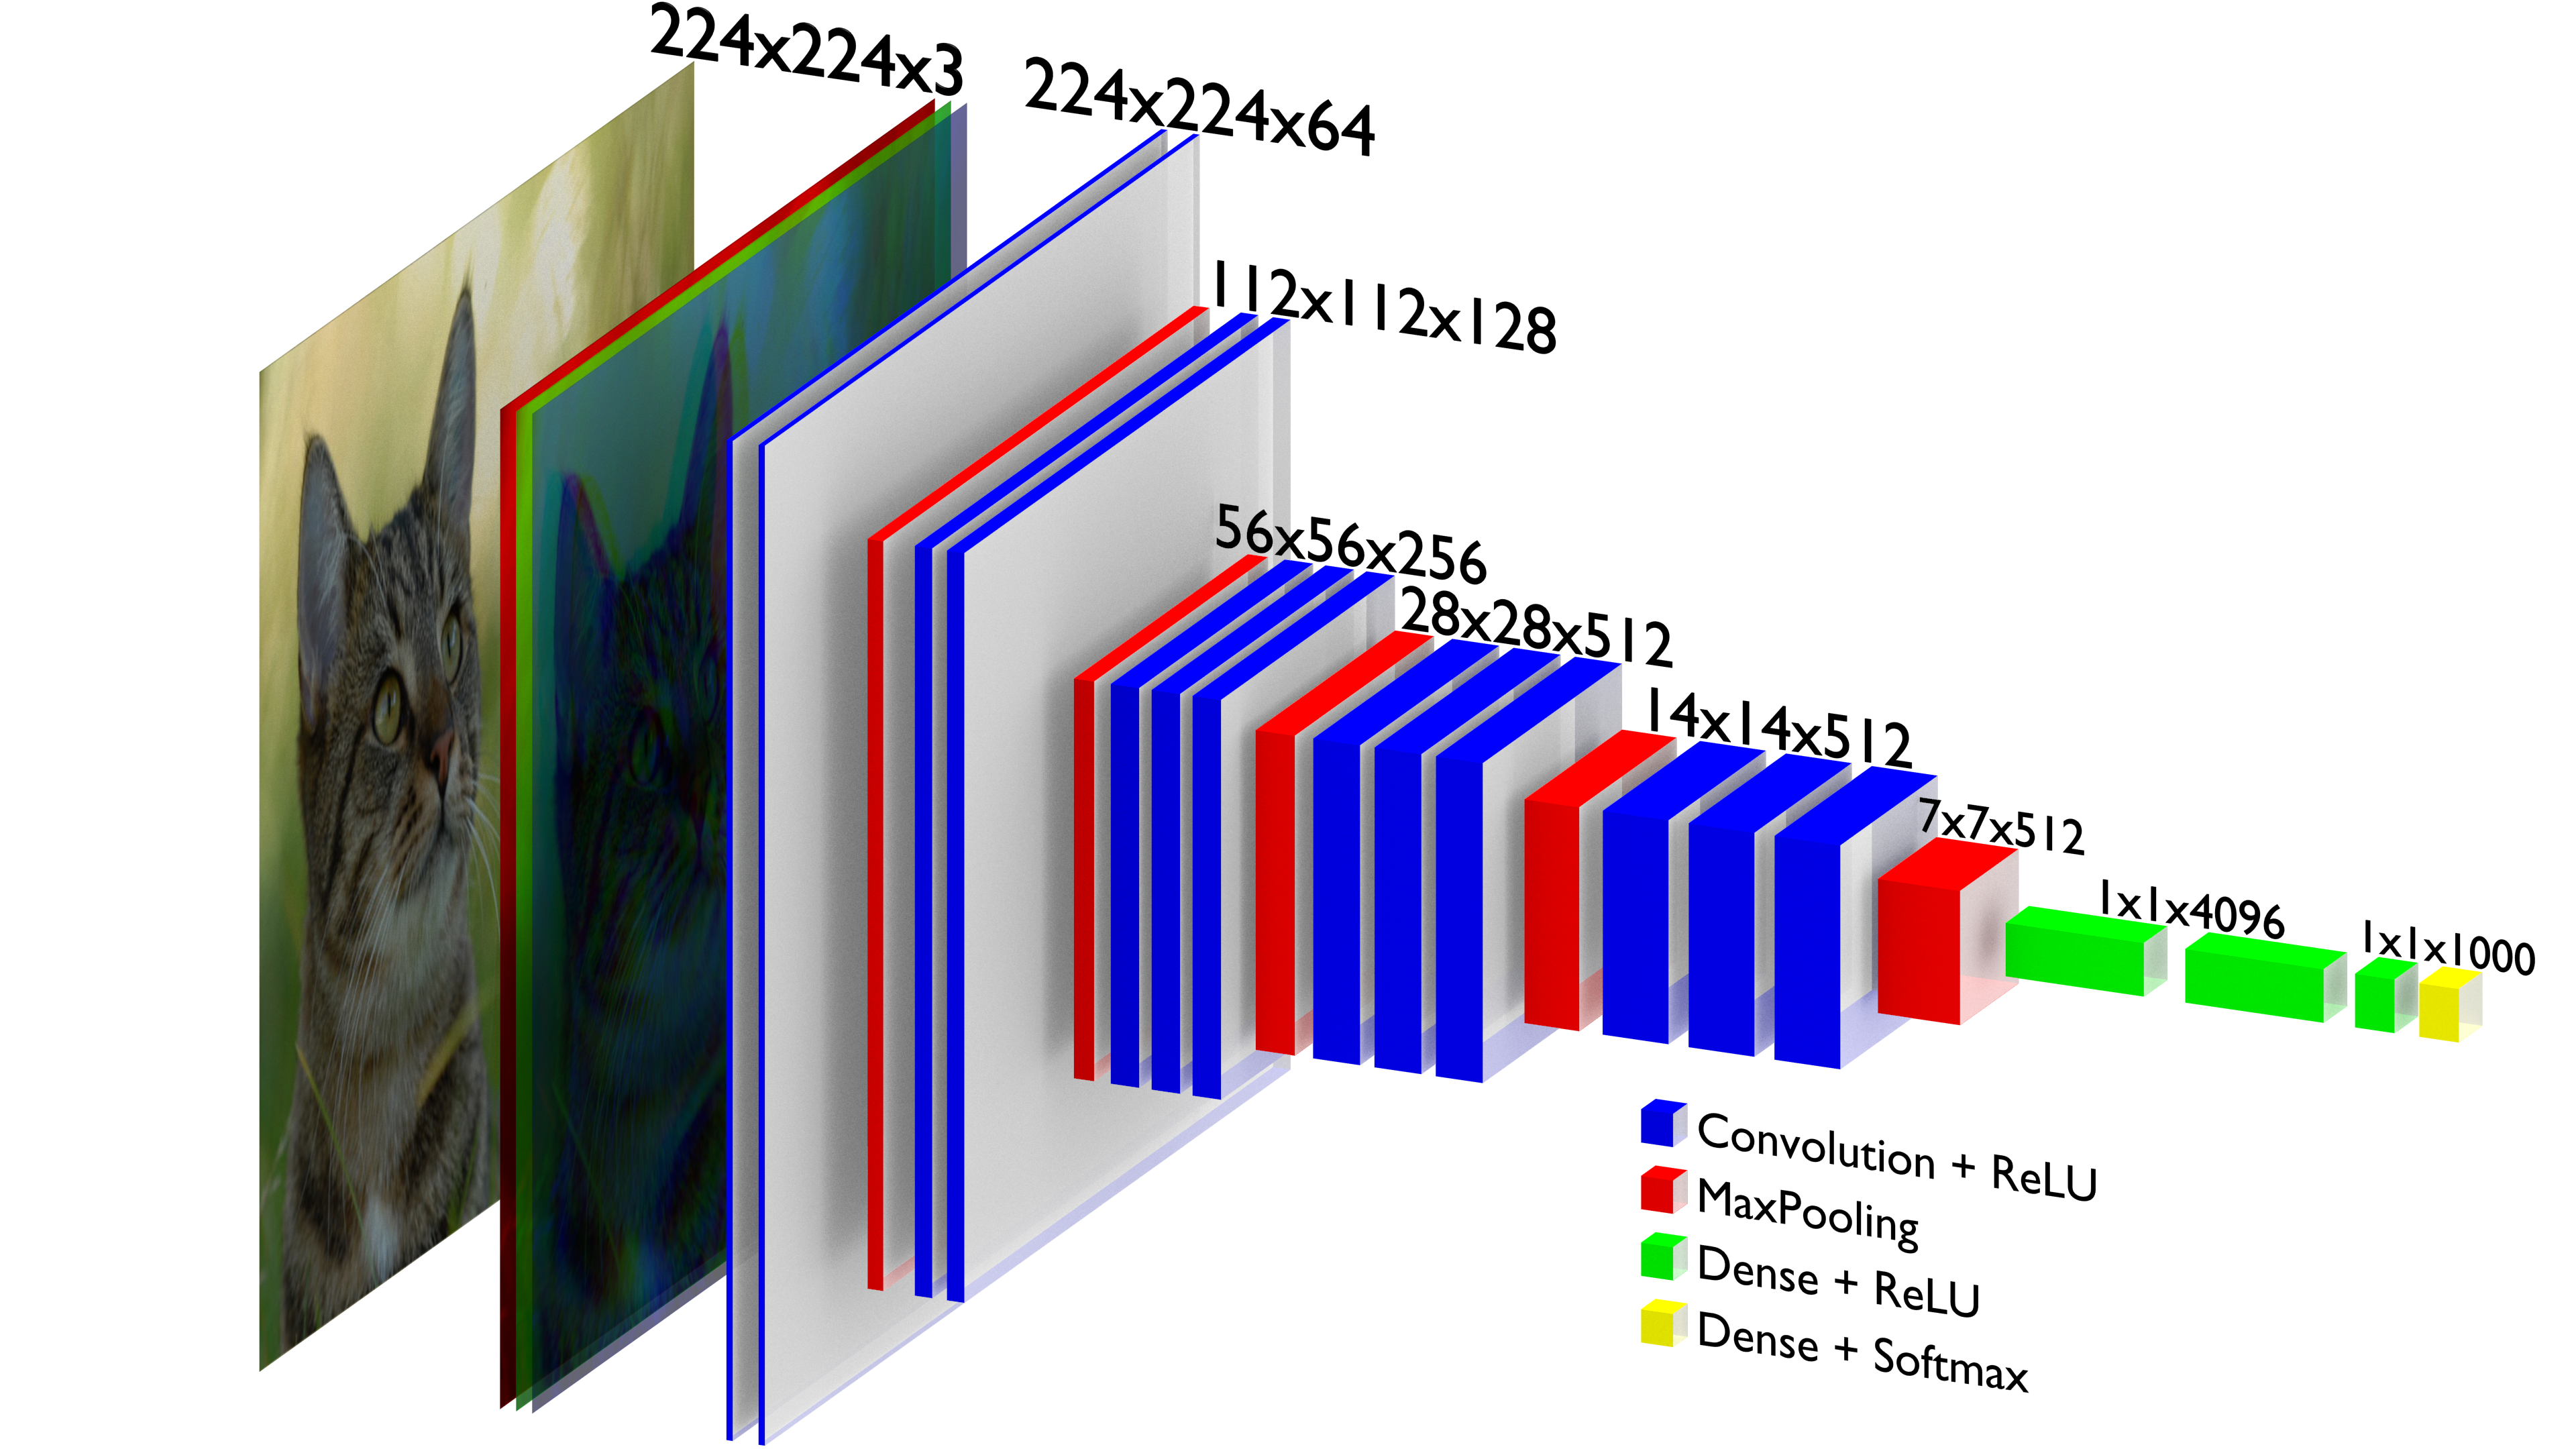
\includegraphics[width=\linewidth]{vgg-16-no-background.png}
	\captionof{figure}{Aufbau des VGG-16}
	\label{fig:vgg-model}
\end{minipage}

\subsection{Dropout Layer}
In unseren CNNs nutzen wir Dropout Layer. Diese deaktivieren zufällig einen festgelegten Anteil der eingehenden Neuronen, setzen ihre Werte also auf 0. Auf diese Weise wird dem Overfitting entgegengewirkt, da das Netzwerk gezwungen ist, viele unterschiedliche Merkmale zu lernen, anstatt nur weniger dominanter.

\section{Daten}
Der verwendete Datensatz stammt von einer Oxford-Studie und besteht ursprünglich aus 102 Klassen. Für unsere Zwecke reduzieren wir den Datensatz ohne spezielle Auswahlkriterien auf 10 Klassen. Die Anzahl der Bilder pro Klasse beschränken wir auf 40 Bilder, um Konsistenz bei der Anzahl der Bilder pro Klasse sicherzustellen. Von den 40 Bildern dienen stets die ersten 5 Bilder als Testbilder und die Übrigen als Vergleichs- oder Trainingsdaten. Beim Training der neuronalen Netze werden 20\%, also 7 der 35 Trainingsbilder, vom Training ausgenommen und als Validierungsbilder verwendet.
\\

\begin{minipage}{.9\linewidth}
\begin{center}
	\includegraphics[scale=.46]{examples2.png}
	\captionof{figure}{Beispiele aus allen Klassen}
\end{center}
\end{minipage}

\subsection{Herausforderungen}
Bei der Klassifikation von Pflanzen bzw. Blüten gibt es einige Herausforderungen. Erstens ist die Region of Interest, in diesem Fall die Blüte, meistens unterschiedlich groß. Dadurch ist teilweise mehr Hintergrund im Bild, andere Male füllt die Blüte fast das gesamte Bild aus. Darüber hinaus wurden die Blüten aus unterschiedlichen Winkeln fotografiert, was ihre Form anders erscheinen lässt. Diese beiden Faktoren verkomplizieren außerdem die Segmentierung.

\section{Methodik}
In diesem Abschnitt werden die Funktionsweisen der implementierten Methoden beschrieben. Klassifikatoren nach klassischem Ansatz sind dabei auf vorher bestimmte Merkmale angewiesen, wohingegen ein CNN eigenständig Merkmale findet.

\subsection{Klassischer Ansatz}
Die im Rahmen dieser Arbeit ausgetesteten Merkmale für den klassischen Ansatz sind die kanalweisen Farbmittelwerte und Farbhistogramme in Verbin\-dung mit einem k-nearest-neighbour Klassifikator sowie das Histogram of Oriented Gradients mit einem neuronalen Netzwerk als Klassifikator.

\subsubsection{Segmentierung}
Um Störeinflüsse zu verringern und die korrekte Klassifikation eines Objektes zu erleichtern ist es manchmal hilfreich das relevante Objekt vom Hintergrund zu trennen. Wir nutzen zu diesem Zweck die Methode des k-means clustering aus \ref{subsec:KMeans_Basics} mit $k=2$.

Die Wahl der initialen Clusterzentren hat beim k-means clustering einen großen Einfluss auf die Qualität der finalen Partitionierung. Da die meisten Blumen nicht bildfüllend aufgenommen wurden, dienen uns die Randpixel des Bildes als Abschätzung für die Farbe des Hintergrunds. Als Farbe des Vordergrunds wählen wir zunächst den Farbdurchschnitt des Bildes. Die ermittelten Farben für den Vorder- und Hintergrund werden als Clusterzentren dem k-means-Algorithmus übergeben, welcher dafür sorgt, dass sich beide einer guten Segmentierung annähern.

Nachdem eine finale Segmentierung gefunden ist, werden die als Hintergrund ermittelten Pixel auf den Farbwert (0,0,0) gesetzt. Aus den Vordergrundpixeln wird die größte zusammenhängende Region ermittelt und das Bild auf diesen Bereich zugeschnitten.

Beispiel 1 in der nachfolgenden Abbildung \ref{fig:segmentation} zeigt ein optimales Resultat der Segmentierung. Die Blüte ist vollständig inkludiert und jeglicher Hintergrund wurde entfernt.

\begin{wrapfigure}[6]{r}{.4\linewidth}
	\raisebox{0pt}[\dimexpr\height-3\baselineskip\relax]{
		\includegraphics[scale=.5]{Segmentierung.png}
	}
	\captionof{figure}{Beispiele für gute und misslungene Segmentierung}
	\label{fig:segmentation}
\end{wrapfigure}
Das zweite Beispiel illustriert hingegen eine misslungene Segmentierung. Die Blume wurde komplett entfernt und statt\-dessen ein Teil des Hintergrunds als Vordergrund erkannt.


\subsubsection{Farben als Merkmale}
Ausschließlich Farbmerkmale eines Bildes zur Klassifikation zu nutzen ist nicht in jedem Fall ein brauchbarerer Ansatz, in der betrachteten Domäne aber durchaus sinnvoll, da schon die Farbe einer Blume allein einen guten Hinweis auf ihre Art gibt.
Ein sehr simpler Deskriptor ist ein 3-Tupel aus den Mittelwerten aller Pixel für jeden Farbkanal. Informationsreicher  ist dagegen ein Farbhistogramm. Dieses unterteilt jeden Farbkanal in eine vorgegebene Anzahl an Stufen auf, in unserem Fall 7 Bins, und zählt die Zahl der Pixel des Bildes, die in einen Bereich fallen. Diese werden anschließend aneinandergereiht. Bei 3 Farbkanälen und 7 Bins pro Kanal besteht der Deskriptor damit aus 3 * 7 = 21 Werten.
Die Klassifikation eines Bildes anhand des Deskriptors erfolgt in beiden Fällen mittels der k-Nearest-Neighbour Methode.

\subsubsection{K-Nearest-Neighbour}
Liegt ein Deskriptor als Vektor vor, kann die k-Nearest-Neighbour Methode verwendet werden, um diesen einer Klasse zuzuordnen. Dazu wird für das einzuordnende Testbild zu jedem Bild der Trainingsdaten die euklidische Distanz der Deskriptoren berechnet und die k-besten Trainingsbilder mit der geringsten Distanz ausgewählt. Aus diesen wird das (oder ggf. eines der) am häufigsten vorkommende(n) Label ermittelt und das zu klassifizierende Bild der entsprechenden Klasse zugeordnet.

\subsubsection{HOG als Merkmal}
Ein etwas andersartiges Merkmal als die vorherigen ist das Histogram of Oriented Gradients, kurz HOG. Dieser Ansatz lässt Farben außen vor und richtet den Fokus stattdessen auf die Kanten innerhalb des Bildes, versucht sich also in der Erkennung von Formen. Bei der Einordnung von Blumen die Form der Blüten zu berücksichtigen ist nachvollziehbar, auch dieser Ansatz scheint daher für die betrachtete Domäne angemessen. 

Bevor wir das HOG eines Bildes berechnen, skalieren wir dieses zunächst auf eine einheitliche Größe. Dies ist notwendig, damit die Deskriptoren der Bilder am Ende die gleiche Länge haben und vergleichbar sind. Außerdem fordert das neuronale Netzwerk, das schlussendlich die Klassifikation übernimmt, eine feste Eingabegröße. In unserer Umsetzung werden die Bilder auf eine Größe von 224 * 224 Pixel skaliert. Anschließend verwenden wir eine Funktion der scikit-image Bibliothek zur Berechnung des HOG wie in \ref{subsec:HOG_Basics} beschrieben. Dabei dienen 1-D Sobelfilter der Form $[-1, 0, 1]$ und $[-1, 0, 1]^T$ der einfachen Berechnung der horizontalen und vertikalen Gradienten \cite{Dalal}\cite{sk_hog}. Aus dem gemeinsamen Gradienten werden bei einer Zellengröße von $14*14$ die Histogramme der $(\frac{224}{14})^2=256$ Zellen mit jeweils neun Behältern für die Orientierungen ermittelt. Die anschließende Normalisierung erfolgt nach der L2-Hys Methode mit einer Blockgröße von $1*1$, also zellenweise ohne Berücksichtigung benachbarter Zellen. L2-Hys skaliert einen Vektor zunächst mittels der euklidischen Distanz (L2-Norm):
$$v_s=\frac{v}{\sqrt{v_1^2 + v_2^2 + ... v_n^3 + \varepsilon^2}}$$
Dabei ist $\varepsilon$ eine kleine Konstante, die Divison durch Null verhindert. Zu\-sätz\-lich zur L2-Normalisierung werden die Werte auf ein Maximum von 0,2 beschnitten und erneut normalisiert \cite{wiki_hog}. Dadurch wird der Einfluss sehr heller Kanten in kontrastreichen Bereichen reduziert.

Für die Klassifikation mit HOGs ist der k-Nearest-Neighbour Klassifikator ungeeignet, da dieser keine Verschiebungen oder Skalierung des Vektors erkennen kann. Wir verwenden daher ein neuronales Netzwerk als Klassifikator. Der Aufbau des Netzes ist in Abbildung \ref{fig:hog-modell} skizziert. Der zuvor berechnete HOG-Deskriptor umfasst 2304 Parameter (256 Zellen mal 9 Richtungen) und bildet die Eingabe für das Netz. Die erste Hidden Layer ist eine Dense Layer mit 1024 Neuronen und ReLU-Aktivierungsfunktion. Nach einer Dropout Layer, die 40\% der Neuronen deaktiviert, folgt eine Dense Layer mit 256 Neuronen und ReLU. Den Schluss bildet eine Dense Layer mit 10 Neuronen, welche die Softmax-Aktivierungsfunktion verwendet.

\begin{minipage}{.92\linewidth}
	\includegraphics[width=\linewidth]{hog-modell.png}
	\captionof{figure}{Klassifikation mit HOG}
	\label{fig:hog-modell}
\end{minipage}

\subsection{Deep Learning Ansatz}
Der Deep Learning Ansatz beschreibt die Verwendung eines CNNs zur Lösung des Problems. Anders als beim klassischen Ansatz werden hierfür keine Merkmale definiert, stattdessen dient das gesamte Bild als Grundlage der Klassifikation.

Die Basis unserer Umsetzung ist das VGG-16 (siehe \ref{subsec:VGG_Basics}) mit den für die ILSVRC-2014 trainierten Gewichten. Dadurch, dass das VGG-16 auf einem sehr umfangreichen Datensatz trainiert wurde, kann es eine viel größere Auswahl an Formen und Objekten erkennen, als es einem auf dem vergleichsweise kleinen Blumendatensatz trainierten CNN je möglich wäre.

Im VGG-16 dienen die Convolutional (Conv) und Pooling Layer der Erkennung von Merkmalen, während die Klassifikation überwiegend von den Dense Layer übernommen wird. Durch Ersetzen der Dense Layer kann die Fähigkeit der Merkmals- und Objekterkennung des VGG-16 auf neue Klassen übertragen werden. Da unser Problem nur zehn Klassen umfasst, nutzen wir zwei kleinere Dense Layer. Außerdem verwenden wir eine Dropout Layer, die 50\% der eingehenden Neuronen zufällig deaktiviert und verhindern soll, dass sich das Netzwerk zu sehr auf wenige, in den Trainingsdaten dominante Merkmale spezialisiert.

Der Aufbau des finalen CNN ist in Abbildung \ref{fig:vgg-modified} dargestellt. Bis auf die ausgetauschten Dense Layer entspricht es dem ursprünglichen VGG-16 (vgl. Abb. \ref{fig:vgg-model} in Abschnitt \ref{subsec:VGG_Basics}). Da wir die vortrainierten Gewichte verwenden, legen wir für das Training auf dem Blumendatensatz fest, dass nur die Layer nach der vierten Max Pooling Layer trainiert werden und die übrigen Layer unverändert bleiben.
\\

\begin{minipage}{.91\linewidth}
	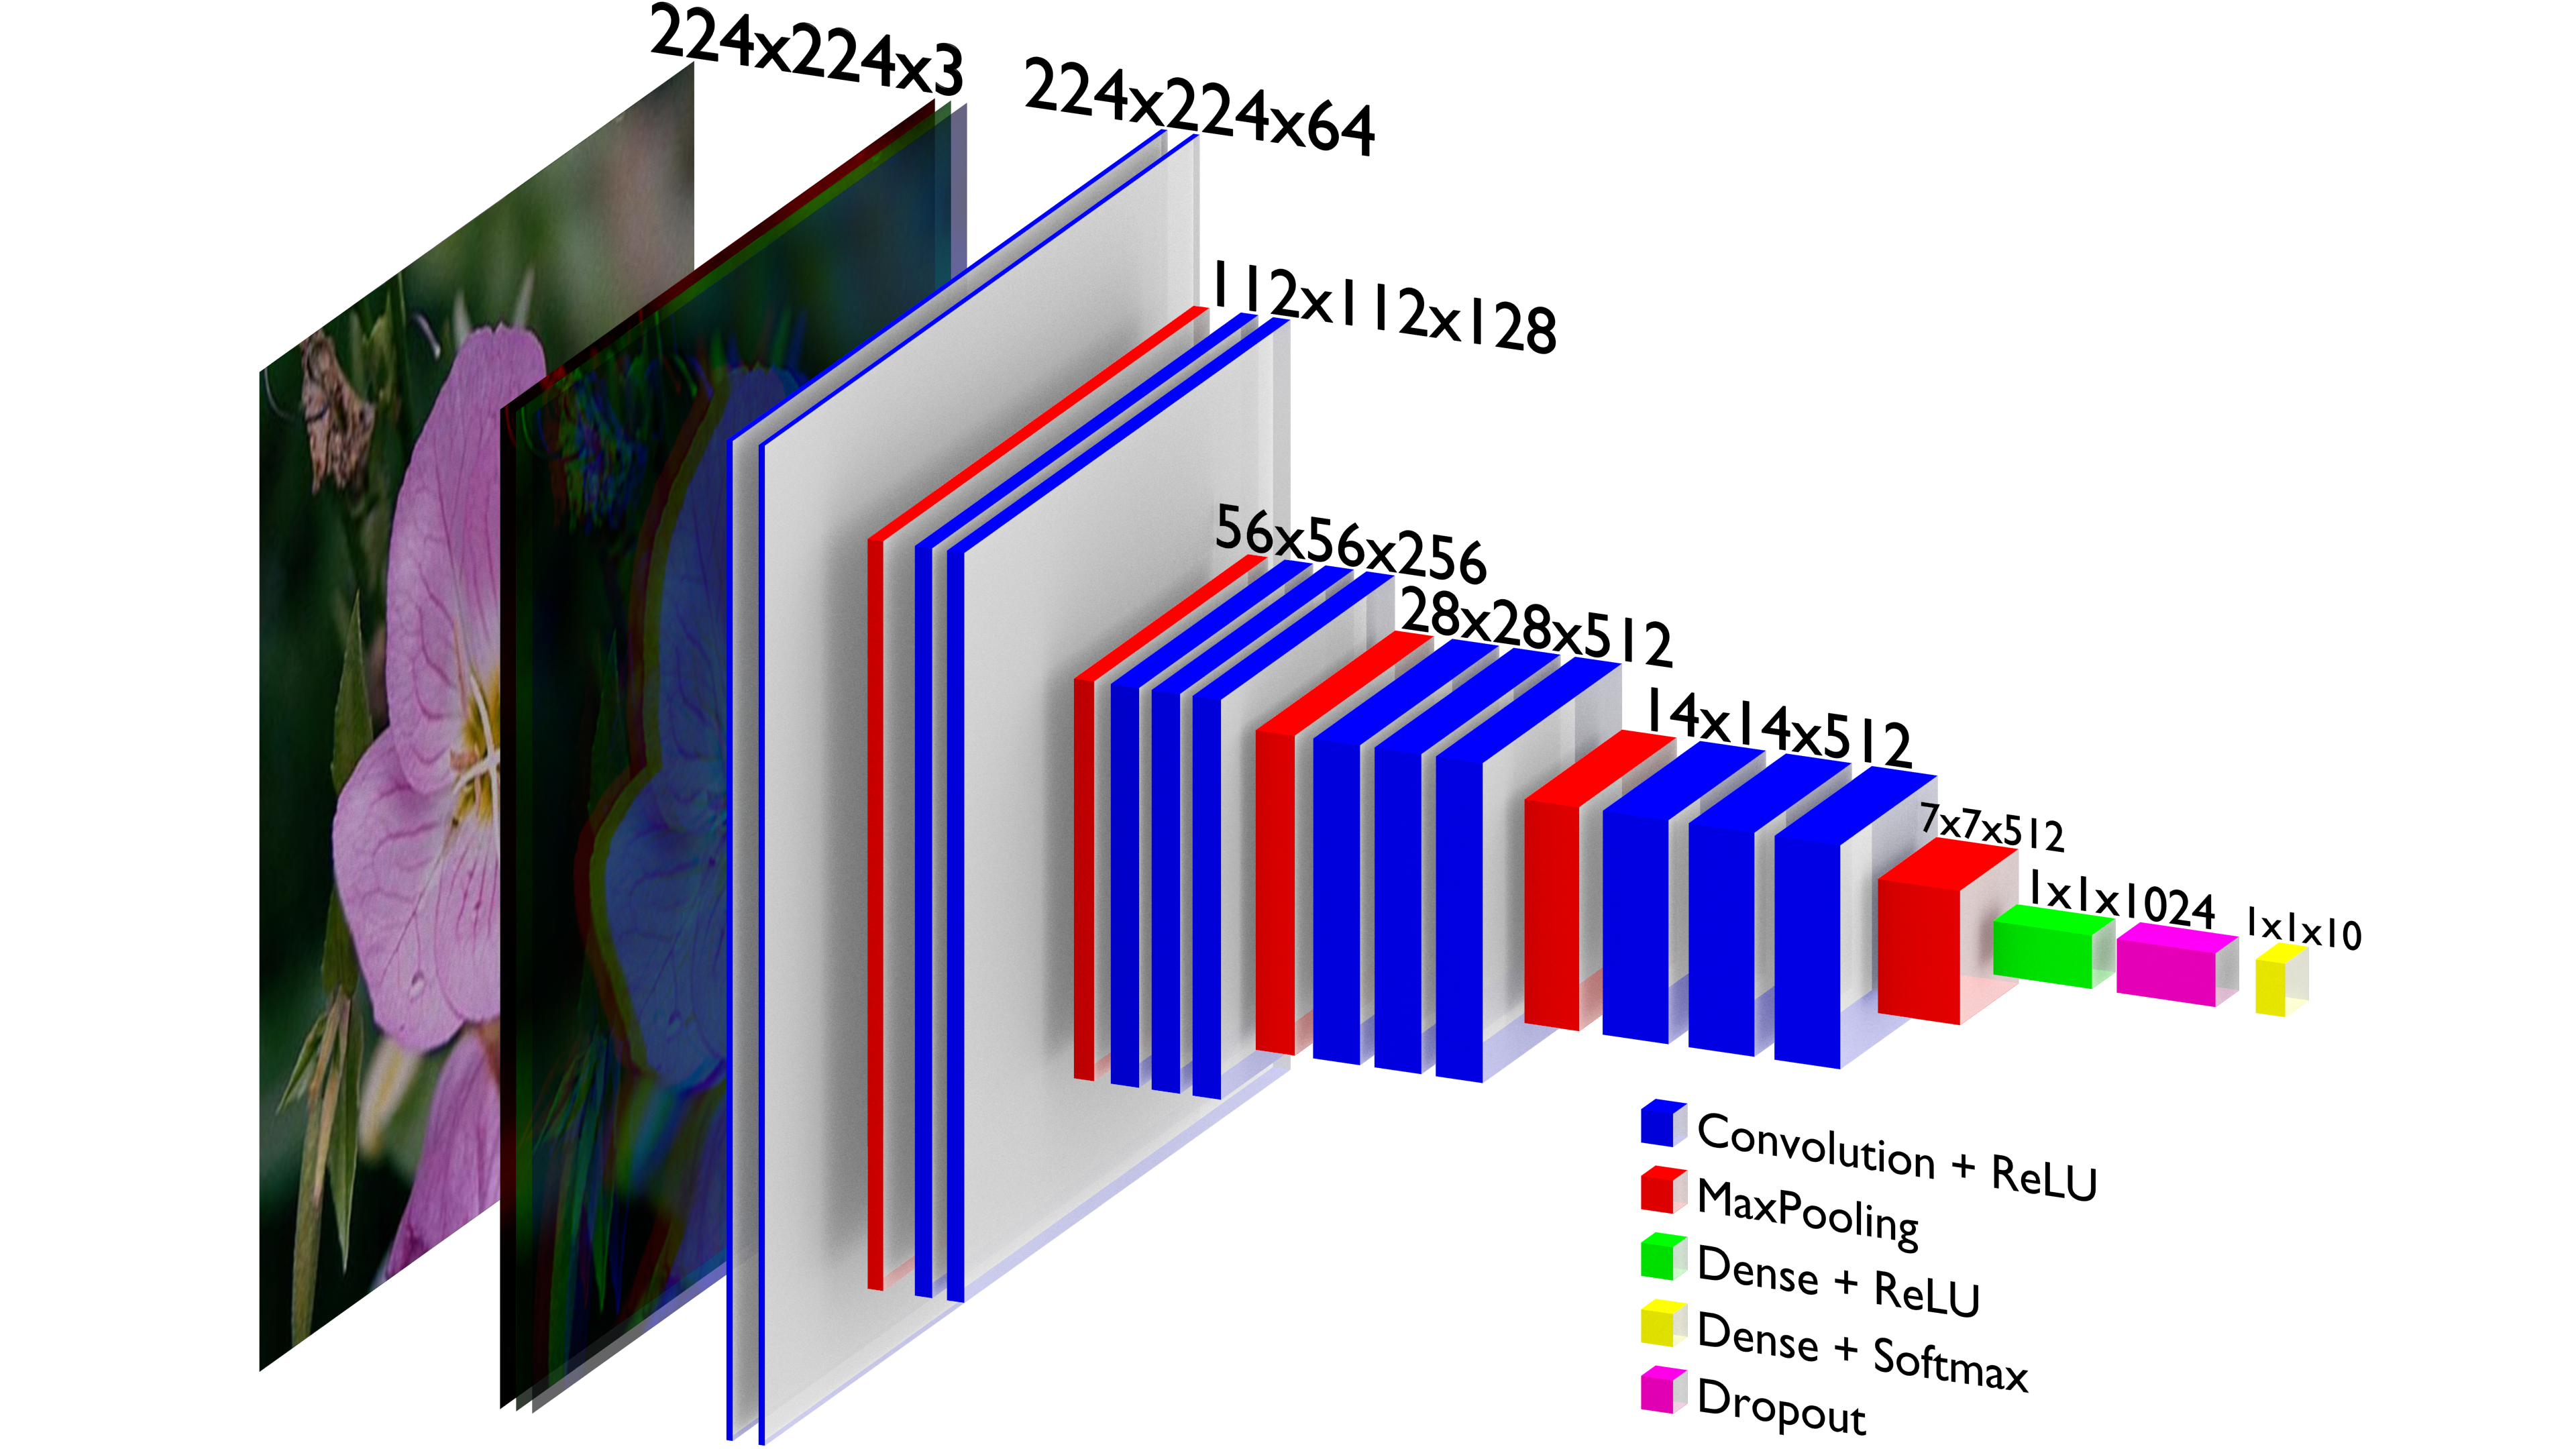
\includegraphics[width=\linewidth]{vgg-modified-no-background.png}
	\captionof{figure}{Aufbau des modifizierten VGG-16}
	\label{fig:vgg-modified}
\end{minipage}

\subsection{Training}
Das Training der neuronalen Netze unterscheidet sich trotz der sehr verschiedenen Architekturen nur unwesentlich. Das Training des CNN erfolgt in Batches von 5, für das HOG beträgt die Batchsize 10. Die anfängliche Learning Rate ist in beiden Fällen $0,001$ und das Momentum $0,9$. Als Loss-Funktion dient die kategorische Kreuzentropie ("Categorical crossentropy") und das Optimierungsverfahren ist der Stochastic Gradient Descent. Durch Early Stopping wird das Training vorzeitig beendet, wenn sich der Validation Loss innerhalb von fünf aufeinanderfolgenden Epochen nicht verbessert. Nach drei Epochen ohne Verbesserung wird die Learning Rate um den Faktor 0,1 reduziert. Von allen Epochen werden die Gewichte der Epoche mit dem besten Validation Loss für das finale Netzwerk gewählt.

\section{Experimente}


\subsection{Klassischer Ansatz}
Die Erkennungsraten der klassischen Verfahren liegen weit hinter denen des Deep Learning Ansatzes. Tabelle \ref{tab:acc__og_edit} listet die Ergebnisse der einzelnen Verfahren auf. Auf den unbearbeiteten Bildern liefert die Verwendung des HOGs mit einer Genauigkeit von 56\% (Durchschnitt aus fünf Durchläufen, Minimum 48\%, Maximum 60\%) die besten Resultate, während die Farbmittelwert-Methode mit einer Erkennungsrate von lediglich 36\% am schlechtesten abschneidet. Bei Verwendung der segmentierten Bilder an Stelle der Originalbilder steigt die Erkennungsrate mit den Mittelwerten auf 54\% und kommt nah an die Ergebnisse des HOG-Verfahren heran. Auch die Farbhistogramme verbessern sich mit den segmentierten Bildern um 6\% von 44 auf 50 Prozent erkannter Blumen. Dabei ist allerdings zu beachten, dass die Leistungsfähigkeit beider Methoden besonders von der farblichen Vielfalt der berücksichtigten Blumenarten abhängt. Außerdem ist die Berechnung der segmentierten Bilder sehr zeitaufwendig und muss daher separat vorbereitet werden. Die Segmentierung von 522 Bildern der zehn Klassen dauerte etwa 1 Stunde und 17 Minuten.

\begin{center}
	\begin{tabular}{c || c | c}
		Merkmal & Originalbilder & Segmentierte Bilder \\ \hline \hline
		Farbmittelwerte & $36\%$ & $54\%$ \\ \hline
		Farbhistogramme & $44\%$ & $50\%$ \\ \hline
		HOG & $56\%$ & $46\%$
	\end{tabular}
	\captionof{table}{Vergleich der Erkennungsraten der originalen und segmentierten Bilder}
	\label{tab:acc__og_edit}
\end{center}

Um die Resultate des klassischen Ansatzes zu verbessern, können die Klassifikatoren in Ensembles kombiniert werden, welche die individuellen Vorhersagen zu einer gemeinsamen Vorhersage vereinen. Soll ein solches Ensemble ein Bild klassifizieren, liefert zunächst jeder Klassifikator eine Wahrscheinlichkeitsverteilung über die Zugehörigkeit des Bildes zu den zehn Klassen. Für die Methoden, die k-nearest-neighbour Klassifikation verwenden, ergibt sich die Wahrscheinlichkeit einer Klasse aus ihrer Häufigkeit in den k nächsten Nachbarn. Bei Verwendung des neuronalen Netzwerks zur Klassifikation wird die Ausgabe der Softmax Layer verwendet. Zur Ermitt\-lung der gemeinsamen Vorhersage vergleichen wir zwei Berechnungsmethoden: Im ersten Fall wird die Vorhersage mit der für sich genommen maxi\-malen Wahrscheinlichkeit (Konfidenz) übernommen, im zweiten Fall wird die Klasse mit der durchschnittlich höchsten Konfidenz in allen Klassifikatoren gewählt.

Die Ergebnisse der Ensembles sind in Tabelle \ref{tab:classic_ensembles} aufgeführt. Ist das HOG Teil des Ensembles sind die Werte über fünf Durchläufe gemittelt und das jeweils beste und schlechteste Ergebnis separat angegeben. In fast allen Szenarien führt die Kombination von Klassifikatoren zu einem Anstieg der Erkennungsraten. Einzig der Zusammenschluss aus Farbhistogrammen und HOG bei Wahl der maximalen Konfidenz verschlechtern das Ergebnis auf 53,6\% im Vergleich zu 56\% nur mit HOG. Die besten Resultate liefert die Verbindung aus Farbmittelwerten und HOG mit durchschnittlich 65,6\% und maximal 70\%. Die zusätzliche Inklusion der Farbhistogramme führt nicht zu einer Verbesserung, teilweise ist sogar das Gegenteil der Fall.

\begin{table}[h]
	\begin{center}
		\begin{tabular}{c | c | c}
			& \multicolumn{2}{c}{Gemeinsame Konfidenz} \\ \cline{2-3}
			Merkmale & Maximum & Durchschnitt \\ \hline \hline
			Farbmittelwerte, Farbhistogramme & $58,0\%$ & $58,0\%$ \\ \hline
			Farbhistogramme, HOG & $53,6\%\hspace{10pt}_{52}^{56}$ & $60,8\%\hspace{10pt}_{54}^{66}$ \\ \hline
			Farbmittelwerte, HOG & $65,6\%\hspace{10pt}_{62}^{70}$ & $65,6\%\hspace{10pt}_{60}^{70}$ \\ \hline
			Farbmittelwert, Farbhistogramme, HOG & $63,6\%\hspace{10pt}_{60}^{68}$ & $65,6\%\hspace{10pt}_{62}^{68}$
		\end{tabular}
	\end{center}
\caption{Genauigkeit bei Kombination der Klassifikatoren}
\label{tab:classic_ensembles}
\end{table}

\begin{wrapfigure}[12]{r}{.4\linewidth}
	\raisebox{0pt}[\dimexpr\height-1.5\baselineskip\relax]{
	\includegraphics[scale=.275]{HOG-Mean_Confusion-Matrix.png}
	}
	\captionof{table}{Confusion Matrix für HOG + Mittelwerte}
	\label{tab:cm_hog_mean}
\end{wrapfigure}
Tabelle \ref{tab:cm_hog_mean} zeigt die Confusion Matrix eines Durchlaufs des besten Modells. Auffällig sind besonders die niedrigen Erkennungsraten der Klassen 4 und 9, aus denen nur eine einzige Blume richtig eingeordnet wurde. Ein Blick auf die Bilder beider Klassen gibt Aufschluss auf die Probleme des Verfahrens. Die Blumen haben alle mehrere Blüten mit relativ komplexen Formen, wodurch die Arbeit des HOG grundsätzlich erschwert wird. Klasse 4 ist außerdem farblich nicht einheitlich, sondern umfasst weiße, pinke, lila und rote Blumen verschiedenster Schattierungen. Dies könnte dem Farbmittelwert-Klassifikator Probleme bereiten. Klasse 9 ist anders als Klasse 4 farblich monoton violett. Sie wurde fälschlicherweise den Klassen 1 und 10 zugeordnet, von denen sich besonders die erste auffällig im Farbton unterscheidet. Beide unterscheiden sich zudem stark in ihrer Blütenform von Klasse 9. Die Problematik könnte in diesem Fall bei der Segmentierung liegen. Auf vielen der segmentierten Bildern aus Klasse 9 sind noch große Teile des Hintergrunds zu sehen. Dadurch wird der Farbdurchschnitt verzehrt, was die fehlerhaften Vorhersagen erklären könnte.



\iffalse
%Confusion Matrix in Tabellenform
\begin{table}[h]
	\begin{center}
		\begin{tabular}{c || c | c | c | c | c | c | c | c | c | c }
			  & 1 & 2 & 3 & 4 & 5 & 6 & 7 & 8 & 9 & 10 \\ \hline \hline
			1 & 3 & 0 & 0 & 0 & 0 & 0 & 1 & 0 & 0 & 1 \\ \hline
			2 & 0 & 5 & 0 & 0 & 0 & 0 & 0 & 0 & 0 & 0 \\ \hline
			3 & 1 & 0 & 4 & 0 & 0 & 0 & 0 & 0 & 0 & 0 \\ \hline
			4 & 0 & 1 & 0 & 0 & 0 & 1 & 1 & 0 & 2 & 0 \\ \hline
			5 & 0 & 0 & 0 & 0 & 5 & 0 & 0 & 0 & 0 & 0 \\ \hline
			6 & 0 & 0 & 0 & 0 & 0 & 5 & 0 & 0 & 0 & 0 \\ \hline
			7 & 0 & 0 & 0 & 0 & 0 & 0 & 5 & 0 & 0 & 0 \\ \hline
			8 & 0 & 0 & 0 & 0 & 0 & 0 & 2 & 3 & 0 & 0 \\ \hline
			9 & 2 & 0 & 0 & 0 & 0 & 0 & 0 & 0 & 1 & 2 \\ \hline
			10 & 0 & 0 & 0 & 0 & 0 & 0 & 0 & 0 & 1 & 4
		\end{tabular}
	\end{center}
\caption{Confusion Matrix für HOG + Mittelwerte}
\label{tab:cm_hog_mean_Old}
\end{table}
\fi

\subsection{Deep Learning Ansatz}
\begin{wrapfigure}[14]{r}{.4\linewidth}
	\raisebox{0pt}[\dimexpr\height-1\baselineskip\relax]{
	\includegraphics[scale=.275]{VGG16_Confusion-Matrix.png}
	}
	\captionof{table}{Confusion Matrix des CNN}
	\label{tab:cm_vgg}
\end{wrapfigure}
Weit bessere Ergebnisse als der klassische Ansatz erzielt das CNN. Nach einem kurzen, 50 Sekunden dauernden Training erreicht das CNN eine Genauigkeit von 100\% auf den Trainings- und 90\% auf den Validierungsbildern. Die Erkennungsrate auf den Testbildern liegt mit 92\% sogar leicht über der Erkennungsrate der Validierungsdaten. Die Confusion Matrix in Tabelle \ref{tab:cm_vgg} zeigt auf, dass die meisten Fehler durch falsche Zuordnung zur Klasse 3 auftraten. Besonders die Einordnung einer Ringelblume aus Klasse 5 in Klasse 3 überrascht in Anbetracht der starken farblichen Abgrenzung.
\\
\begin{wrapfigure}[16]{l}{.8\linewidth}
	\raisebox{0pt}[\dimexpr\height-0\baselineskip\relax]{
	\includegraphics[scale=.4]{vgg_errors.png}
	}
	\captionof{figure}{Die vom CNN falsch klassifizierten Bilder}
	\label{fig:vgg-misses}
\end{wrapfigure}

In Abbildung \ref{fig:vgg-misses} sind die falsch klassifizierten Bilder aufgelistet. Die Bilder der weiß-violetten Blumen aus Klasse 9 unterscheiden sich von anderen ihrer Klasse vor allem durch die Orientierung der Blumen, die orange Blume durch die Zahl der abgebildeten Blüten und die rosafarbene Blume hebt sich in ihrer Farbe vom Rest ihrer Klasse ab. Für alle vier fehlen somit Referenzen in der Trainingsdatenbank. Für drei der vier Bilder gilt außerdem, dass das richtige Label an zweiter Stelle in den besten Vorhersagen steht. Beides weist darauf hin, dass eine umfassendere Datenbasis die Performance des Modells verbessern könnte. Diese Annahme bestätigt sich, wenn wir unseren Datensatz durch Data Augmentation künstlich vergrößern. Indem wir die Bilder zufällig bis zu 90$^\circ$ rotieren, vertikal spiegeln und zoomen generieren wir uns einen Datensatz, der 20 Mal größer ist als zuvor. Die Trainingszeit erhöht sich dadurch auf etwa acht Minuten. Das Ergebnis ist eine Erkennungsrate von 97,14\% auf den Validierungsbildern und 98\% auf den Testbildern. Einzig das rechte obere Bild in Abbildung \ref{fig:vgg-misses} aus Klasse 9 ist noch der falschen Klasse zugeordnet.



\section{Fazit}
Zusammenfassend lässt sich sagen, dass der klassische Ansatz mit einer Genauigkeit von maximal 70\% um 28\% schlechter ist als der CNN Ansatz. Die Ergebnisse lassen sich aber nur bedingt vergleichen, da das CNN dem klassischen Ansatz ein vorheriges Training auf tausenden Bildern voraus hat. Mit einer deutlich größeren Datenbasis und unter Nutzung neuer Merkmale sollten auch mit dem klassischen Ansatz gute Erkennungsraten möglich sein. Es sollten Merkmale betrachtet werden, die auch sehr bunte Blumenarten wie die Klasse 4 gut repräsentieren können. Außerdem sollten bessere Segmentierungsverfahren entwickelt werden, um Probleme mit den Hintergründen wie bei Klasse 9 zu verhindern. Die größte Schwierigkeit mit dem klassischen Ansatz ist aber der Entwicklungsaufwand. Das Finden und Implementieren von Merkmalen, das Vergleichen mit der Datenbank bei Verwendung des k-Nearest-Neighbour-Algorithmus, das Training des neuronalen Netzwerks und die Segmentierung erfordern mit einer immer größeren Datenbasis mehr und mehr Aufwand. Im Gegensatz dazu ist die Verwendung des VGG schnell und einfach möglich und profitiert von Beginn an vom Training auf einer umfangreichen Datenbank. Unser CNN hat nach einem Training mit nur 28 Bildern pro Klasse nur 4 Bilder falsch klassifiziert. Diese sind Sonderfälle ihrer Klassen ohne gute Referenzbilder. Mit einem größeren Trainingsdatensatz sollten sich problemlos Erkennungsraten nahe der 100\% erzielen lassen, wie die Ergebnisse der Data Augmentation zeigen.

Für unser erstes Anwendungsbeispiel aus der Einleitung, der Unkrautsbekämpfung, sind eigentlich nur zwei Klassen notwendig. Es muss nur die Klasse der angebauten Pflanze von der Klasse des Unkrauts, welche alle anderen Pflanzen umfasst, unterschieden werden. Diese Aufgabe sollte mit beiden Ansätzen gut machbar sein.
Für das zweite Anwendungsbeispiel der Analyse kompletter Ökosysteme sind deutlich mehr Klassen als 10 erforderlich. Je nach Detailgrad ist hierfür die Verwendung eines oder mehrerer Deep-CNNs der beste Ansatz. Unterstützend könnte eine App entwickelt werden, die Hobbygärtnern und anderen Interessierten die Identifikation ihnen unbekannter Pflanzen anhand eines einfachen Fotos ermöglicht, und auf diese Weise neue Bilder für die Datenbank generiert.

\begin{thebibliography}{99}

	\bibitem{ImageNet2014}{Olga Russakovsky*, Jia Deng*, Hao Su, Jonathan Krause, Sanjeev Satheesh, Sean Ma, Zhiheng Huang, Andrej Karpathy, Aditya Khosla, Michael Bernstein, Alexander C. Bergand Li Fei-Fei. (* = equal contribution) ImageNet Large Scale Visual Recognition Challenge. IJCV, 2015
	\\ http://www.image-net.org/challenges/LSVRC/2014/index}
	
	\bibitem{VGG16_Paper}{Karen Simonyan and Andrew Zisserman, Visual Geometry Group, Department of Engineering Science, University of Oxford, "Very Deep Convolutional Networks for Large-Scale Image Recognition", 2015}
	
	\bibitem{Dalal}{Dalal, N. and Triggs, B., “Histograms of Oriented Gradients for Human Detection,” IEEE Computer Society Conference on Computer Vision and Pattern Recognition, 2005, San Diego, CA, USA}
	
	\bibitem{ocv_hog}{https://www.learnopencv.com/histogram-of-oriented-gradients/(05.09.2019)}
	
	\bibitem{sk_hog}{https://scikit-image.org/docs/dev/api/skimage.feature.html\#skimage.feature.hog (05.09.2019)}
	
	\bibitem{wiki_hog}{https://en.wikipedia.org/wiki/Histogram\_of\_oriented\_gradients (20.09.2019)}
	
\end{thebibliography}


\end{document}

